\chapter{Clustering on Graphs}

Finding clusters is an important task in many disciplines, whether to uncover hidden functional similarities in protein interaction networks, to compress data, or to improve ecommerce recommendations. The second part of this thesis studies how we can use neural networks to do clustering on graphs.  

\begin{figure}[H]
\begin{center}
  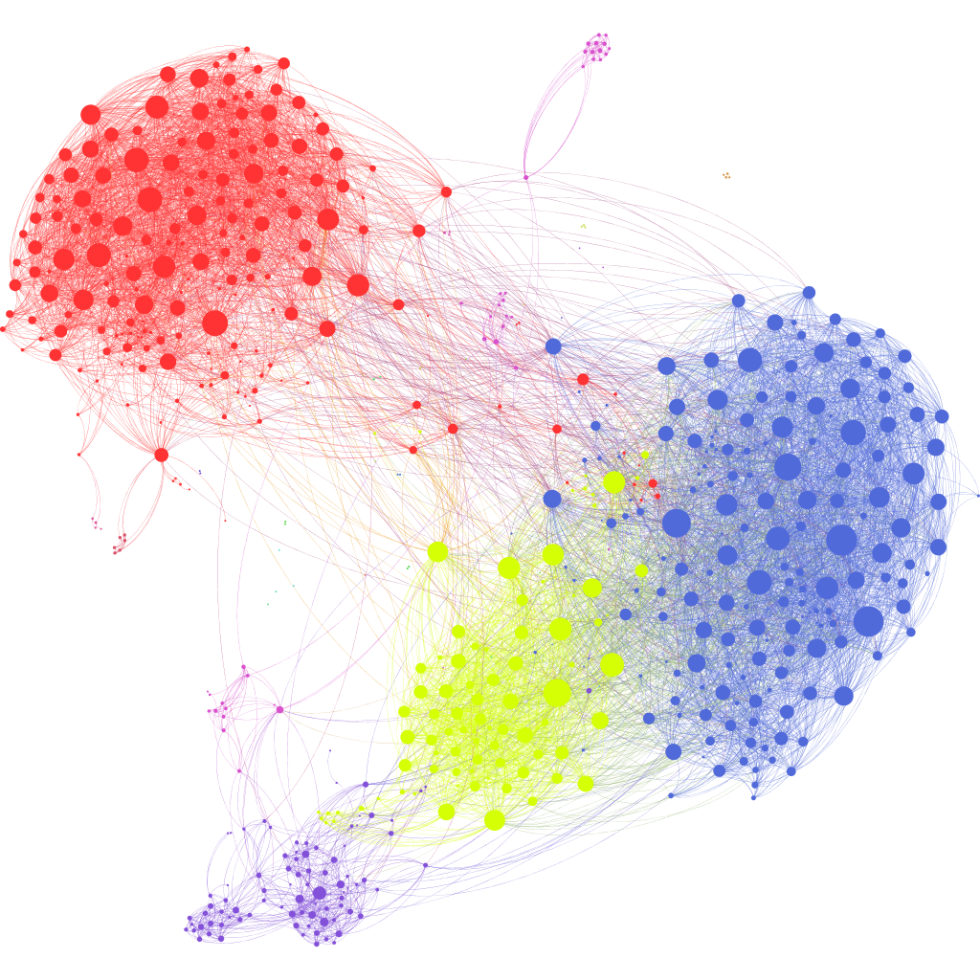
\includegraphics[scale=0.13]{social_network.png}
  \caption{A sampling of a Facebook friend network.\cite{social_network}}
  \label{fig:socialnet}
 \end{center}
\end{figure}

Clustering is a procedure applied to datasets in which we output a community label for each vertex.  All vertices that have the same label are referred to as cluster. Points within a cluster share some kind of similarity, more so with each other than with points outside the cluster. The definition is not precise because clustering can span the spectrum between supervised (eg. community detection with ground truth) and unsupervised problems (eg. data exploration). Graph clustering is the clustering procedure applied to a dataset that has graph structure. The goal here is to use the extra topological information of the network to do clustering and inform choices of similarity measures.


Applied to social networks, clustering is oftentimes referred to as community detection. The procedure can be data driven or model driven.  In the former we let the  features in datasets motivate definitions of similarity metrics and even suggest ground truth.  In the latter, a probabilistic generative model is often used, where the generative mechanism defines the ground truth communities.  The two approaches are not unrelated.  Generative models, for instance, are designed to mimic statistics of real graphs.  The Stochastic Blockmodel is an example of such a benchmark artificial dataset and we will discuss it in detail.  




\begin{figure}
\begin{center}
  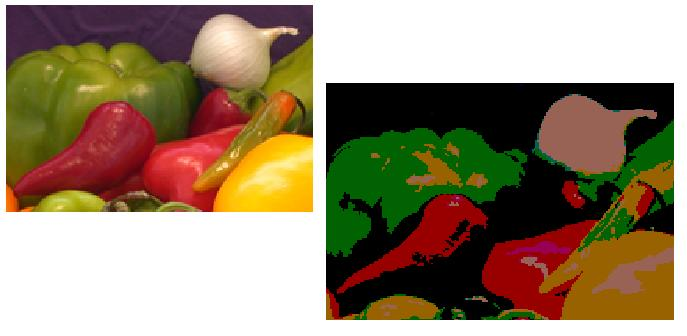
\includegraphics[scale=0.35]{image_segmentation.jpg}
  \caption{A result of image segmentation.\cite{image_seg}}
  \label{fig:seg}
 \end{center}
\end{figure}

\begin{figure}
\begin{center}
  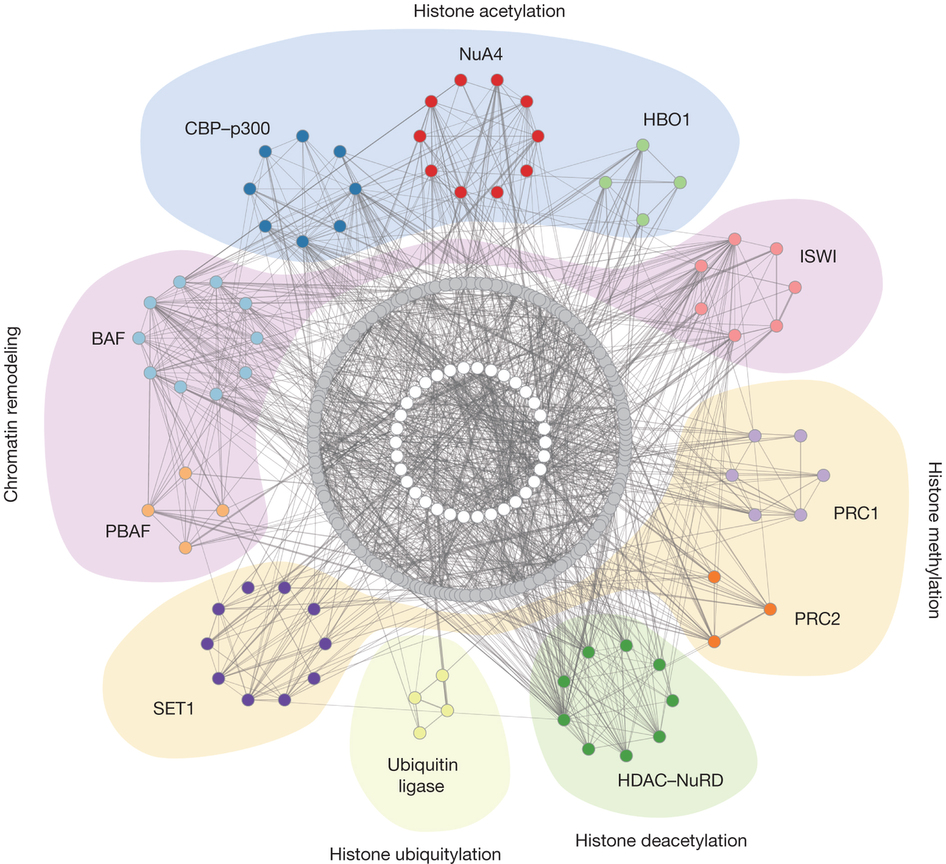
\includegraphics[scale=0.20]{protien_network.jpg}
  \caption{A protein to protein interaction network.\cite{protein}}
  \label{fig:protien}
 \end{center}
\end{figure}



The benefit of the neural network approach is that we do not have to choose what algorithm to use via heuristics or local statistics gathered from the network.  Instead it is data driven.  The model will learn by gradient descent, fitting the best parameters given the distributions of the graphs it learns from.  We will first go over the well studied Stochastic Blockmodel and some of the algorithmic challenges of community detection in this model. Then we will introduce the Graph Neural Network, a model we designed that can successfully do clustering on the SBM, even in the hardest regimes.  We will present our experimental results in the last section.  

